\documentclass[a4paper,9pt,twocolumn,twoside,]{pinp}

%% Some pieces required from the pandoc template
\providecommand{\tightlist}{%
  \setlength{\itemsep}{0pt}\setlength{\parskip}{0pt}}

% Use the lineno option to display guide line numbers if required.
% Note that the use of elements such as single-column equations
% may affect the guide line number alignment.

\usepackage[T1]{fontenc}
\usepackage[utf8]{inputenc}

% pinp change: the geometry package layout settings need to be set here, not in pinp.cls
\geometry{layoutsize={0.95588\paperwidth,0.98864\paperheight},%
  layouthoffset=0.02206\paperwidth, layoutvoffset=0.00568\paperheight}

\definecolor{pinpblue}{HTML}{185FAF}  % imagecolorpicker on blue for new R logo
\definecolor{pnasbluetext}{RGB}{101,0,0} %



\title{Predicting Obesity Using DASL Dataset (R10-09)}

\author[]{460352996 470066919 480145820 480407614}

  \affil[]{GitHub code repository is
\href{https://github.sydney.edu.au/awon6941/DATA2002-M4.git}{here}}

\setcounter{secnumdepth}{0}

% Please give the surname of the lead author for the running footer
\leadauthor{460352996 470066919 480145820 480407614}

% Keywords are not mandatory, but authors are strongly encouraged to provide them. If provided, please include two to five keywords, separated by the pipe symbol, e.g:
 \keywords{  Obesity |  Regression |  Correlation |  Prediction  }  

\begin{abstract}
Excess weight, especially obesity, has become an epidemic in the 21st
century. This study aims to investigate an alternative method to
determine ``overweight'' individuals oppose to body fat percentage. Two
alternative indicators are considered - BMI and body density. The
results showed that BMI can be explained the best using simple body
measurement and the measurement on abdomen is the most important
predictor in estimating all three methods. A simpler predictive model
for obesity has been developed using measurements on chest, abdomen and
bicep. Limitations and implications are discussed.
\end{abstract}

\dates{This version was compiled on \today} 

% initially we use doi so keep for backwards compatibility
% new name is doi_footer

\pinpfootercontents{A Research on Obesity}

\begin{document}

% Optional adjustment to line up main text (after abstract) of first page with line numbers, when using both lineno and twocolumn options.
% You should only change this length when you've finalised the article contents.
\verticaladjustment{-2pt}

\maketitle
\thispagestyle{firststyle}
\ifthenelse{\boolean{shortarticle}}{\ifthenelse{\boolean{singlecolumn}}{\abscontentformatted}{\abscontent}}{}

% If your first paragraph (i.e. with the \dropcap) contains a list environment (quote, quotation, theorem, definition, enumerate, itemize...), the line after the list may have some extra indentation. If this is the case, add \parshape=0 to the end of the list environment.


\hypertarget{introduction}{%
\subsection{Introduction}\label{introduction}}

Excess weight is the new epidemic of the 21st century and has resulted
in many significant health and economic consequences for the global
population (Stein and Colditz, 2004). In Australia, the obesity epidemic
has spread drastically as 1 in 3 adults are classified as overweight or
obese (Australian Institute of Health and Welfare, 2019). Researches
have shown that this epidemic is more common in males than females and
hence, BYU Human Performance Research Centre has collected data from 250
men of various age and obtained estimates of the percentage of body fat
through underwater weighing and various body circumference measurements
(Rahman and Harding, 2013; DASL, n.d.). As body fat percentage is
difficult to calculate in real life, the value for body fat percentage
was derived from body density using the Siri's 1956 equation (DASL,
n.d.).

\hypertarget{data-cleaning-and-processing}{%
\subsubsection{1.1 Data cleaning and
processing}\label{data-cleaning-and-processing}}

The DASL dataset contain 16 variables including body density, age, body
fat percentage and body measurements. The dataset has already been
cleaned and for the purpose of this analysis, an additional variable -
BMI, has been added where
\[ BMI = \frac{Weight (lbs)*703}{Height(in)^2} \]

\hypertarget{sampling-method}{%
\subsubsection{1.2 Sampling Method}\label{sampling-method}}

Few details were provided with regards to the sampling method. However,
from looking at the dataset, there is a gender bias as the epidemic
question is one related to both genders, yet only males were involved in
the sample. This suggests that any analysis based on this dataset cannot
be applied to the whole population but only the male population.

\hypertarget{analysis}{%
\subsection{Analysis}\label{analysis}}

The analysis approach can be broken down into three steps.

\hypertarget{step-1}{%
\subsubsection{Step 1}\label{step-1}}

Using multiple regression, firstly determine the number of body
measurements that is significant in building an accurate prediction
model for the three obesity indicators (Body Fat Percentage, BMI and
Body Density) individually and how much variation can be explained using
only body measurements to examine the ease of calculation.

\hypertarget{step-2}{%
\subsubsection{Step 2}\label{step-2}}

Compare the end results to determine the best indicator given that body
measurements are the only available variables. In each sample, a
relative importance test will also be run to determine which body
measurement is relatively the most important.

\hypertarget{step-3}{%
\subsubsection{Step 3}\label{step-3}}

Using BMI as the obesity indicator, a binary indicator will be added to
differentiate the sample into overweight individuals (1) and
non-overweight individuals (0). A logistic regression is run on the
binary indicator with significant variables that we have identified
throughout research in order to build a simpler model to determine the
odds of an individual being obese.

\hypertarget{multiple-regression}{%
\subsection{Multiple Regression}\label{multiple-regression}}

\hypertarget{analysis-1}{%
\subsubsection{Analysis}\label{analysis-1}}

A correlation matrix is firstly drawn to show the general interactive
correlation between variables.

\begin{center}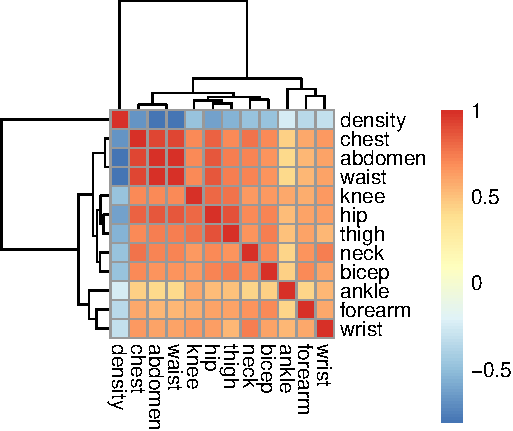
\includegraphics{Executive_Report_files/figure-latex/unnamed-chunk-1-1} \end{center}

\(\textbf{Figure 1:}\textit{ Correlation Matrix}\)

Notably, waist, chest and abdomen are highly correlated, and this may be
due to the fact that they are from a similar body area. Hence, body
measurements that are from similar areas are classified and linked
together using the above graph.

All three obesity indicators follow a similar procedure for multiple
regression analysis.

Backward stepwise model was used for Body Fat and BMI where a full model
was selected at the start. The least informative variables were dropped
using AIC until only the most relevant variables remain and a final
fitted model is achieved. A forward variable selection method was used
for body density and a null model was selected at the beginning with
subsequent addition of the most statistically significant variable. The
final fitted model is formed when no further addition is required.

For the analysis of BMI, a transformation using log was required.
However, as BMI is measured in unit increase, the interpretation of
percentage changed is unreasonable. Hence, the non-transformed model was
used as the final fitted model.

Assumptions for normality and homoskedasticity were checked via
residuals plots and QQ plot and the relative importance of the remaining
variables is illustrated using the predictor plots.

\hypertarget{results}{%
\subsubsection{Results}\label{results}}

The final fitted models for the three obesity indicators were: \[ 
\begin{aligned}
&(1) \hat{Body Fat} = 1.52 -0.3965Neck - 0.128Chest\\
&+ 1.01805Abdomen -0.28758Hip + 0.26Bicep -1.55084Wrist\\
&(2) \hat{BMI} = -10.94 +0.161Chest + 0.127Abdomen\\
&+ 0.050Hip + 0.150Thigh - 0.23Knee + 0.115Forearm\\
&(3) \hat{Body Density} = 1.1104052 + 0.0019085 Neck\\
&- 0.0022064Abdomen + 0.0011314 Hip - 0.0006094 Thigh\\
\end{aligned}
\]

All three QQ plots show straight lines and this satisfies the normality
assumption. However, the residual plots showed a slight variation for
all three indicators, but given that the residual units were quite
small, it is acceptable for the current analysis (Appendix A).

Overall, abdomen is relatively the most important measurement in
predicting all three obesity indicators and this result was expected as
it corresponds to the previous correlation matrix analysis (Appendix B).

BMI was identified as the best obesity indicator given only body
measurements as 90.2\% of its variation can be explained using solely
body measurements compared to 73.5\% for Body Fat Percentage and 70.4\%
for Body Density.

\hypertarget{logistic-regression}{%
\subsection{Logistic Regression}\label{logistic-regression}}

\hypertarget{analysis-2}{%
\subsubsection{Analysis}\label{analysis-2}}

A binary logistic regression was used to calculate the probability of a
person being overweight where overweight is indicated by a BMI greater
or equal to 25. Similar to the multiple regression analysis, a backward
stepwise selection method is used to determine a final classification
model.

Using the model, the probability of an individual being obese is then
derived using a confusion matrix where its performance as a predictive
model is evaluated.

\hypertarget{results-1}{%
\subsubsection{Results}\label{results-1}}

The final classification model is \[
\begin{aligned}
logit(p)=log(\frac{p}{1-p})=-75.89380+0.37854Chest\\ +0.27128Abdomen+0.22381Thigh
\end{aligned}
\]

The results of this model are visualised by Figure 2 through the sigmoid
function. The predicted values to probabilities are mapped between 0 and
1. For predictions of 0.5 and above, these are classified as people who
are overweight. Whereas predictions of below 0.5 are classified as
people who are non-overweight.

\begin{center}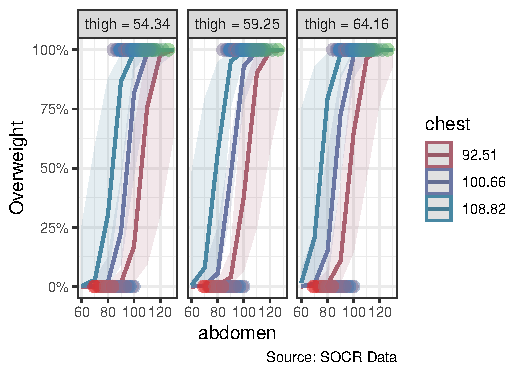
\includegraphics{Executive_Report_files/figure-latex/unnamed-chunk-2-1} \end{center}

\(\textbf{Figure 2:}\textit{Predicted values of Overweight}\)

A confusion matrix is created to derive the performance of our
classification model.

\begin{ShadedResult}
\begin{verbatim}
#            Reference
#  Prediction   0   1
#           0 117  12
#           1   8 113
\end{verbatim}
\end{ShadedResult}

The accurate and inaccurate predictions are the diagonal and
non-diagonal values respectively. For this model, there are 117 + 113
accurate predictions, and 12 + 8 are inaccurate predictions.

The model has a sensitivity, ability to correctly identify those who are
overweight, of 93.6\%; and a specificity of 90.4\%, which is the ability
to correctly identify those who are non-overweight.

Along with an accuracy of 92\%, we summarise that this new simplified
model is, therefore, a good predictive model.

A decision tree on the variables abdomen and chest is represented by
Appendix C. Out of a total of 250 observations, 96\% of people with a
chest circumference greater or equal to 101.55cm are overweight. Also,
of the people with a chest circumference less than 101.55cm, those with
an abdomen circumference greater or equal to 92.6cm are 72\% likely to
be overweight. On the other hand, those with an abdomen circumference
less than 92.6cm are 92\% likely to be non-overweight.

\hypertarget{limitations}{%
\subsection{Limitations}\label{limitations}}

\begin{center}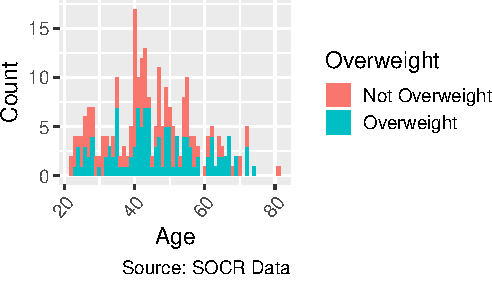
\includegraphics{Executive_Report_files/figure-latex/unnamed-chunk-4-1} \end{center}

\(\textbf{Figure 3:}\textit{Obesity across different age groups}\)

\hypertarget{gender-bias}{%
\subsubsection{4.1 Gender bias}\label{gender-bias}}

The data is taken from 250 males without any record of females.
Therefore, the result of this analysis can only be applied to the male
population rather than the entire population, which will limit the use
of the analysis.

\hypertarget{age-range}{%
\subsubsection{4.2 Age range}\label{age-range}}

Majority of the participants are males between the age of 40-50. This is
a potential bias in the sample that can compromise the prediction
accuracy on younger or older males.

\hypertarget{multicollinearity}{%
\subsubsection{4.3 Multicollinearity}\label{multicollinearity}}

Several variables from the dataset are highly dependent, with the most
significant correlation between waist and abdomen. In a QQ-Plot, all
points are closely sitting on the line. Hence, during model selection,
waist was dropped to prevent multicollinearity.

\hypertarget{conclusion}{%
\subsection{Conclusion}\label{conclusion}}

Through multiple regression and variable selection, a fitted model with
solely body measurements was determined for each of the three obesity
indicators. Using \(R^2\), BMI was identified as the best indicator as
it has the highest proportion of variance that can be explained using
only body measurements.

Abdomen was the most important body measurement for determining obesity
because for all three indicators, it ranked the highest in terms of
relative importance in prediction.

By separating the dataset with the binary variable for over-weight
individuals, a simplified prediction model with 92\% accuracy was built.
The simplified model contains three body measurements - chest, abdomen
and thigh, and should be relatively simpler to measure.

\newpage

\hypertarget{reference-list}{%
\subsection{Reference List}\label{reference-list}}

\hypertarget{section}{%
\subsubsection{1.}\label{section}}

Australian Institute of Health and Welfare (AIHW). (2019). Overweight \&
obesity. Australian Government. Retrieved from
\url{https://www.aihw.gov.au/reports-data/behaviours-risk-factors/overweight-obesity/overview}

\hypertarget{section-1}{%
\subsubsection{2.}\label{section-1}}

DASL. (n.d.). Bodyfat. DASL. Retrieved from
\url{https://dasl.datadescription.com/datafile/bodyfat}

\hypertarget{section-2}{%
\subsubsection{3.}\label{section-2}}

Rahman, A., \& Harding, A. (2013). Prevalence of overweight and obesity
epidemic in Australia: some causes and consequences.~JP Journal of
Biostatistics,~10(1), 31-48.

\hypertarget{section-3}{%
\subsubsection{4.}\label{section-3}}

Stein, C. J., \& Colditz, G. A. (2004). The epidemic of obesity.~The
Journal of Clinical Endocrinology \& Metabolism,~89(6), 2522-2525.

\hypertarget{section-4}{%
\subsubsection{5.}\label{section-4}}

Avinash, N. (2018). Understanding Logistic Regression in
Python.~DataCamp. Retrieved from
\url{https://www.datacamp.com/community/tutorials/understanding-logistic-regression-python}

\hypertarget{section-5}{%
\subsubsection{6.}\label{section-5}}

Nagesh S. C. (n.d.). Real world implementation of Logistic
Regression.~Medium. Retrieved from
\url{https://towardsdatascience.com/real-world-implementation-of-logistic-regression-5136cefb8125}

\hypertarget{appendixes}{%
\subsection{Appendixes}\label{appendixes}}

\hypertarget{appendix-a}{%
\subsubsection{Appendix A}\label{appendix-a}}

Multiple Regression: Assumption Checking in the order of Body Fat
Percentage, BMI and Body Density

\begin{center}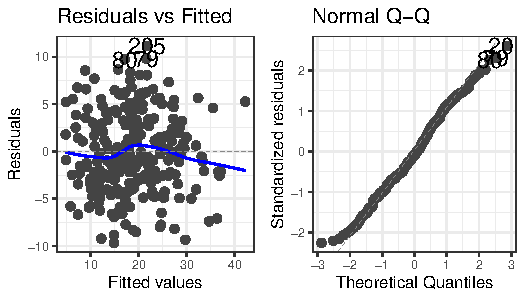
\includegraphics{Executive_Report_files/figure-latex/unnamed-chunk-5-1} \end{center}

\begin{center}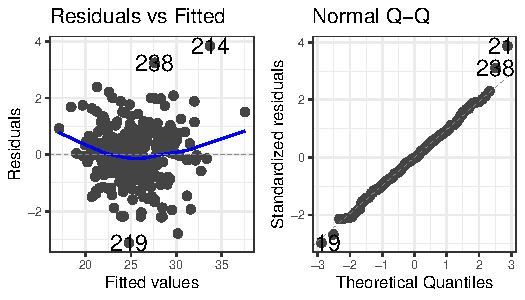
\includegraphics{Executive_Report_files/figure-latex/unnamed-chunk-5-2} \end{center}

\begin{center}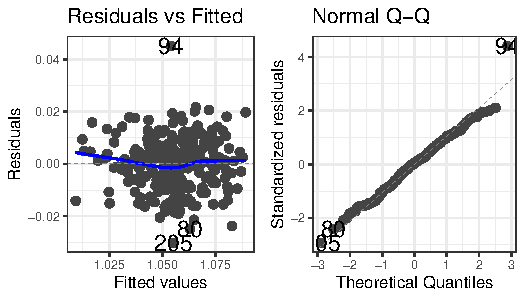
\includegraphics{Executive_Report_files/figure-latex/unnamed-chunk-5-3} \end{center}

\hypertarget{appendix-b}{%
\subsubsection{Appendix B}\label{appendix-b}}

Multiple Regression: Relative Importance of Predictors in the order of
Body Fat Percentage, BMI and Body Density

\begin{ShadedResult}
\begin{verbatim}
#            Weights
#  wrist    4.038431
#  bicep    7.746760
#  neck     8.238378
#  hip     16.313788
#  chest   21.795458
#  abdomen 41.867184
\end{verbatim}
\end{ShadedResult}
\begin{ShadedResult}
\begin{verbatim}
#            Weights
#  forearm  9.021850
#  knee     9.080285
#  thigh   15.075099
#  hip     17.245099
#  abdomen 24.705834
#  chest   24.871833
\end{verbatim}
\end{ShadedResult}
\begin{ShadedResult}
\begin{verbatim}
#           Weights
#  neck    11.06366
#  thigh   13.82063
#  hip     19.73563
#  abdomen 55.38008
\end{verbatim}
\end{ShadedResult}

\hypertarget{appendix-c--}{%
\subsubsection{Appendix C -}\label{appendix-c--}}

Decision Tree on Abdomen and Chest variables

\begin{center}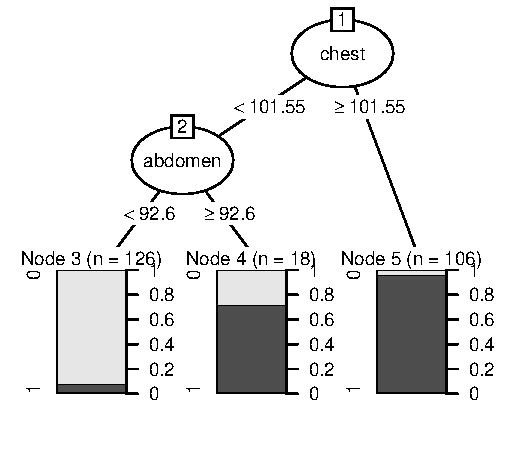
\includegraphics{Executive_Report_files/figure-latex/unnamed-chunk-7-1} \end{center}

%\showmatmethods


\bibliography{pinp}
\bibliographystyle{jss}



\end{document}

